\documentclass{ltjsarticle}
\RequirePackage{luatex85}
\usepackage[utf8]{inputenc}
\usepackage[dvipdfmx]{color}
\usepackage{enumerate}
\usepackage{here}
\usepackage{amsthm}
\usepackage{amsfonts}
\usepackage{amsmath}
\usepackage{amssymb}
\usepackage{latexsym}
\usepackage{ytableau}
\usepackage{docmute}
\usepackage{mathtools}
\usepackage{xr}
\usepackage{tikz}
\usetikzlibrary{intersections, calc, arrows.meta}
\usepackage[all]{xy}
%\usepackage[dvipdfmx]{graphicx}
%\usepackage{hyperref}
%\usepackage{pxjahyper}



\theoremstyle{definition}
\newtheorem{defin}{定義}[subsection]
\newtheorem{theo}[defin]{定理}
\newtheorem{cor}[defin]{系}
\newtheorem{prop}[defin]{命題}
\newtheorem{lemm}[defin]{補題}
\newtheorem{notice}[defin]{注意}
\newtheorem{eg}[defin]{例}
\newtheorem{fact}[defin]{事実}


\renewcommand{\labelenumi}{(\roman{enumi})}


\newcommand{\invlimit}{\mathop{\lim_{\longleftarrow}}}
\newcommand{\dirlimit}{\mathop{\lim_{\longrightarrow}}}
\newcommand{\ind}{\text{Ind}}
\newcommand{\Hom}{\text{Hom}}
\newcommand{\tr}{\text{tr}}
\newcommand{\id}[1]{\text{id}_{#1}}
\newcommand{\sgn}{\mathrm{sgn}}
\newcommand{\res}[1]{\text{Res}_{#1}}
\newcommand{\generated}[1]{\langle\:#1\:\rangle}
\newcommand{\im}{\text{Im }}
\newcommand{\rank}{\text{rank }}
\newcommand{\del}[2]{\frac{\partial #1}{\partial #2}}
\newcommand{\delsametwo}[2]{\frac{\partial^2 #1}{\partial #2^2}}
\newcommand{\delothertwo}[3]{\frac{\partial^2#1}{\partial#2\partial#3}}
\newcommand{\ddel}[2]{\frac{\partial}{\partial #2}#1}
\newcommand{\ddelsametwo}[3]{\frac{\partial^2}{\partial #2^2}#1}
\newcommand{\ddelothertwo}[3]{\frac{\partial^2}{\partial#2\partial#3}#1}
\newcommand{\simneq}{\not\simeq}
\newcommand{\transpose}[1]{^t\!#1}
\newcommand{\ie}{\text{i.e.}}
\newcommand{\inv}[1]{#1^{-1}}
\newcommand{\real}{\mathbb{R}}
\newcommand{\complex}{\mathbb{C}}
\newcommand{\integer}{\mathbb{Z}}
\newcommand{\quotient}{\mathbb{Q}}
\newcommand{\natnum}{\mathbb{N}}
\newcommand{\proj}{\mathbb{P}}
\newcommand{\affine}{\mathbb{A}}
\newcommand{\tensor}[3]{#1\otimes_#2#3}
\newcommand{\map}[3]{#1:#2\rightarrow#3}
\newcommand{\aut}[2]{\mathrm{Aut}_{#1} (#2)}
\newcommand{\hommoph}[2]{\mathrm{Hom}_{#1}(#2)}
\newcommand{\gl}{\text{GL}}
\newcommand{\End}{\text{End}}
\newcommand{\set}[2]{\left\{\:#1\:\middle|\:#2\:\right\}}
\newcommand{\pmat}[1]{\begin{pmatrix} #1
\end{pmatrix}}
\newcommand{\vmat}[1]{\begin{vmatrix} #1
\end{vmatrix}}
\newcommand{\bmat}[1]{\begin{bmatrix} #1
\end{bmatrix}}
\newcommand{\br}{\vskip\baselineskip}
\newcommand{\Lie}{\text{Lie}}
\newcommand{\Sym}{\text{Sym}}
\newcommand{\Alt}{\text{Alt}}
\newcommand{\ch}{\text{ch}}
\newcommand{\diag}{\text{diag}}
\newcommand{\comb}[2]{_{#1}C_{#2}}
\newcommand{\codim}{\text{codim}\:}
\newcommand{\yd}[1]{\ydiagram{#1}}

\title{aaa}
\author{}
\date{}


\begin{document}
\maketitle

\begin{figure}[H]
  \centering
  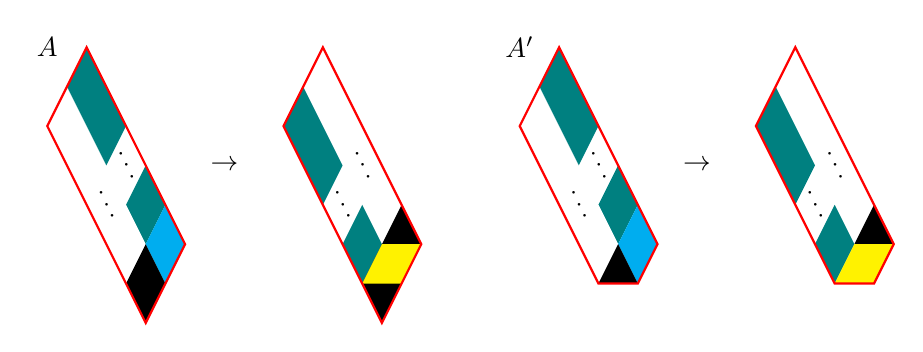
\begin{tikzpicture}
    \begin{scope}
      \fill[teal] (0,0)-- ++(2/4,-2/2)-- ++(-1/4,-1/2)-- ++(-2/4,2/2)--cycle;
      \fill[white] (-1/4,-1/2)-- ++(2/4,-2/2)-- ++(-1/4,1/2)-- ++(-2/4,2/2)--cycle;

      \node[font=\small] at (2/4 - 2/8 + 0.05,-4/2 + 0.1) {\rotatebox{-25}{$\ddots$}};
      \node[font=\small] at (2/4 + 0.05,-3/2 + 0.1) {\rotatebox{-25}{$\ddots$}};
      \fill[teal] (3/4,-3/2)-- ++(1/4,-1/2)-- ++(-1/4,-1/2)-- ++(-1/4,1/2)--cycle;
      \fill[white] (2/4,-4/2)-- ++(1/4,-1/2)-- ++(-1/4,-1/2)-- ++(-1/4,1/2)--cycle;

      \fill[cyan] (4/4,-4/2)-- ++(1/4,-1/2)-- ++(-1/4,-1/2)-- ++(-1/4,1/2)--cycle;
      \fill[black] (3/4,-5/2)-- ++(1/4,-1/2)-- ++(-1/4,-1/2)-- ++(-1/4,1/2)--cycle;
      
      \draw[thick,red] (0,0)-- ++(5/4,-5/2)-- ++(-2/4,-2/2)-- ++(-5/4,5/2)--cycle;
      \node at (-1/2,0) {$A$};
      \node at (3/4 + 1,-3/2) {$\rightarrow$};
    \end{scope}

    \begin{scope}[xshift=3cm]
      \fill[white] (0,0)-- ++(2/4,-2/2)-- ++(-1/4,-1/2)-- ++(-2/4,2/2)--cycle;
      \fill[teal] (-1/4,-1/2)-- ++(2/4,-2/2)-- ++(-1/4,-1/2)-- ++(-2/4,2/2)--cycle;

      \node[font=\small] at (2/4 - 2/8 + 0.05,-4/2 + 0.1) {\rotatebox{-25}{$\ddots$}};
      \node[font=\small] at (2/4 + 0.05,-3/2 + 0.1) {\rotatebox{-25}{$\ddots$}};
      \fill[white] (3/4,-3/2)-- ++(1/4,-1/2)-- ++(-1/4,-1/2)-- ++(-1/4,1/2)--cycle;
      \fill[teal] (2/4,-4/2)-- ++(1/4,-1/2)-- ++(-1/4,-1/2)-- ++(-1/4,1/2)--cycle;

      \fill[black] (4/4,-4/2)-- ++(1/4,-1/2)-- ++(-2/4,-2/2)-- ++(-1/4,1/2)--cycle;
      \fill[yellow] (3/4,-5/2)-- ++(1/2,0)-- ++(-1/4,-1/2)-- ++(-1/2,0)--cycle;
      
      \draw[thick,red] (0,0)-- ++(5/4,-5/2)-- ++(-2/4,-2/2)-- ++(-5/4,5/2)--cycle;
    \end{scope}




    \begin{scope}[xshift = 6cm]
      \fill[teal] (0,0)-- ++(2/4,-2/2)-- ++(-1/4,-1/2)-- ++(-2/4,2/2)--cycle;
      \fill[white] (-1/4,-1/2)-- ++(2/4,-2/2)-- ++(-1/4,1/2)-- ++(-2/4,2/2)--cycle;

      \node[font=\small] at (2/4 - 2/8 + 0.05,-4/2 + 0.1) {\rotatebox{-25}{$\ddots$}};
      \node[font=\small] at (2/4 + 0.05,-3/2 + 0.1) {\rotatebox{-25}{$\ddots$}};
      \fill[teal] (3/4,-3/2)-- ++(1/4,-1/2)-- ++(-1/4,-1/2)-- ++(-1/4,1/2)--cycle;
      \fill[white] (2/4,-4/2)-- ++(1/4,-1/2)-- ++(-1/4,-1/2)-- ++(-1/4,1/2)--cycle;

      \fill[cyan] (4/4,-4/2)-- ++(1/4,-1/2)-- ++(-1/4,-1/2)-- ++(-1/4,1/2)--cycle;
      \fill[black] (3/4,-5/2)-- ++(1/4,-1/2)-- ++(-1/2,0)--cycle;
      
      \draw[thick,red] (0,0)-- ++(5/4,-5/2)-- ++(-1/4,-1/2)--++(-1/2,0)-- ++(-4/4,4/2)--cycle;
      \node at (-1/2,0) {$A'$};
      \node at (3/4 + 1,-3/2) {$\rightarrow$};
    \end{scope}

    \begin{scope}[xshift=9cm]
      \fill[white] (0,0)-- ++(2/4,-2/2)-- ++(-1/4,-1/2)-- ++(-2/4,2/2)--cycle;
      \fill[teal] (-1/4,-1/2)-- ++(2/4,-2/2)-- ++(-1/4,-1/2)-- ++(-2/4,2/2)--cycle;

      \node[font=\small] at (2/4 - 2/8 + 0.05,-4/2 + 0.1) {\rotatebox{-25}{$\ddots$}};
      \node[font=\small] at (2/4 + 0.05,-3/2 + 0.1) {\rotatebox{-25}{$\ddots$}};
      \fill[white] (3/4,-3/2)-- ++(1/4,-1/2)-- ++(-1/4,-1/2)-- ++(-1/4,1/2)--cycle;
      \fill[teal] (2/4,-4/2)-- ++(1/4,-1/2)-- ++(-1/4,-1/2)-- ++(-1/4,1/2)--cycle;

      \fill[black] (4/4,-4/2)-- ++(1/4,-1/2)-- ++(-1/2,0)--cycle;
      \fill[yellow] (3/4,-5/2)-- ++(1/2,0)-- ++(-1/4,-1/2)--++(-1/2,0)--cycle;
      
      \draw[thick,red] (0,0)-- ++(5/4,-5/2)-- ++(-1/4,-1/2)--++(-1/2,0)-- ++(-4/4,4/2)--cycle;
    \end{scope}

    

    
  \end{tikzpicture}
  \caption{パーツに対する変形.赤枠の辺上にあるラベルは変形後も保たれているこ.} \label{parts deformation}
\end{figure}

\end{document}